%%%%%%%%%%%%%%%%%%%%%%%%%%%%%%%%%%%%%%%%%%%%%%%%%%%%%%%%%%%%%%%%%%%%%%%%%%%%%%%
%%%%%%%%%%%%%%%%%%%%%%%%%%%%%%%%%%%%%%%%%%%%%%%%%%%%%%%%%%%%%%%%%%%%%%%%%%%%%%%

\begin{frame}
\frametitle{Задача}

Разработка мобильного оконного менеджера для ОС Linux для отображения пользовательских приложений на платформе Raspberry Pi Zero
\\
Разработка в рамках проекта "Смартфон XXon"
\end{frame}

%%%%%%%%%%%%%%%%%%%%%%%%%%%%%%%%%%%%%%%%%%%%%%%%%%%%%%%%%%%%%%%%%%%%%%%%%%%%%%%
%%%%%%%%%%%%%%%%%%%%%%%%%%%%%%%%%%%%%%%%%%%%%%%%%%%%%%%%%%%%%%%%%%%%%%%%%%%%%%%

\begin{frame}
\frametitle{Архитектура проекта}

\begin{figure}
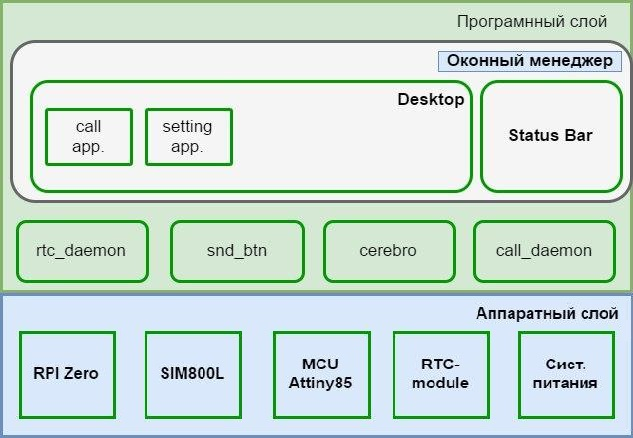
\includegraphics[width=\linewidth]{architecture}
\end{figure}

\end{frame}

%%%%%%%%%%%%%%%%%%%%%%%%%%%%%%%%%%%%%%%%%%%%%%%%%%%%%%%%%%%%%%%%%%%%%%%%%%%%%%%
%%%%%%%%%%%%%%%%%%%%%%%%%%%%%%%%%%%%%%%%%%%%%%%%%%%%%%%%%%%%%%%%%%%%%%%%%%%%%%%

\begin{frame}
\frametitle{Задачи, решаемые в рамках проекта}

\begin{itemize}
\item разработка аппаратной платформы на основе RPi Zero
\item установка и конфигурирование ОС для RPi Zero
\item разработка стека драйверов для комплектующих
\item разработка сервисного слоя (в виде демонов UNIX)
\item \textbf{разработка мобильного оконного менеджера}
\item разработка клиентских приложений
\end{itemize}

\end{frame}

%%%%%%%%%%%%%%%%%%%%%%%%%%%%%%%%%%%%%%%%%%%%%%%%%%%%%%%%%%%%%%%%%%%%%%%%%%%%%%%
%%%%%%%%%%%%%%%%%%%%%%%%%%%%%%%%%%%%%%%%%%%%%%%%%%%%%%%%%%%%%%%%%%%%%%%%%%%%%%%

\begin{frame}
\frametitle{Постановка задачи}

\begin{itemize}
\item Оконный менеджер для RPi Zero
\item Поддержка системных приложений:
	\begin{itemize}
	\item[-] Строка состояния
	\item[-] Рабочий стол
	\end{itemize}
\item Конфигурируемость (для указания системных приложений)
\item Корректная отрисовка разных типов окон
\item Возможность запуска из экранного менеджера
\item Обработка комбинаций клавиш
\item \textit{Возможность перемещения и изменения размеров окна}
\end{itemize}

\end{frame}

%%%%%%%%%%%%%%%%%%%%%%%%%%%%%%%%%%%%%%%%%%%%%%%%%%%%%%%%%%%%%%%%%%%%%%%%%%%%%%%
%%%%%%%%%%%%%%%%%%%%%%%%%%%%%%%%%%%%%%%%%%%%%%%%%%%%%%%%%%%%%%%%%%%%%%%%%%%%%%%

\begin{frame}
\frametitle{Wayland}

\begin{figure}[h!]
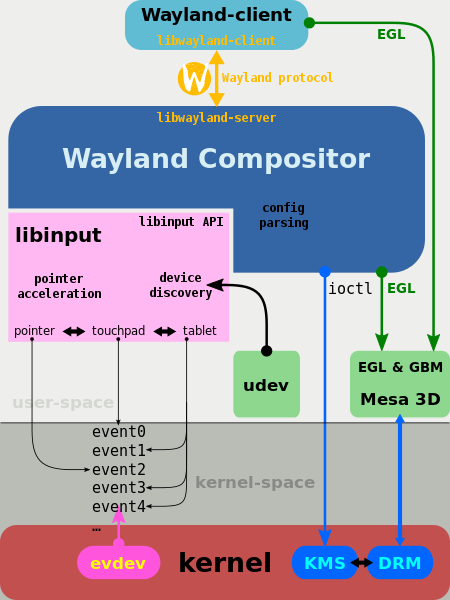
\includegraphics[height=80mm]{waylandArchitechture}
\end{figure}

\end{frame}

%%%%%%%%%%%%%%%%%%%%%%%%%%%%%%%%%%%%%%%%%%%%%%%%%%%%%%%%%%%%%%%%%%%%%%%%%%%%%%%
%%%%%%%%%%%%%%%%%%%%%%%%%%%%%%%%%%%%%%%%%%%%%%%%%%%%%%%%%%%%%%%%%%%%%%%%%%%%%%%

\begin{frame}
\frametitle{WLC}

WLC --- библиотека-композитор для Wayland. На основе этой библиотеки реализовано несколько оконных менеджеров и других библиотек. Их примеры:
\begin{itemize}
\item Тайлинговый оконный менеджер Sway
\item Модульный композитор orbment
\item Модульный ОМ fireplace
\end{itemize}

\end{frame}

%%%%%%%%%%%%%%%%%%%%%%%%%%%%%%%%%%%%%%%%%%%%%%%%%%%%%%%%%%%%%%%%%%%%%%%%%%%%%%%
%%%%%%%%%%%%%%%%%%%%%%%%%%%%%%%%%%%%%%%%%%%%%%%%%%%%%%%%%%%%%%%%%%%%%%%%%%%%%%%

\begin{frame}
\frametitle{Тестовый стенд}

Для выполнения работы использовалось два тестовых стенда:
\begin{itemize}
\item Платформа Raspberry Pi 1 с ОС ArchLinux
\item Виртуальная машина с Arch Linux
\end{itemize}

\end{frame}

%%%%%%%%%%%%%%%%%%%%%%%%%%%%%%%%%%%%%%%%%%%%%%%%%%%%%%%%%%%%%%%%%%%%%%%%%%%%%%%
%%%%%%%%%%%%%%%%%%%%%%%%%%%%%%%%%%%%%%%%%%%%%%%%%%%%%%%%%%%%%%%%%%%%%%%%%%%%%%%

\begin{frame}
\frametitle{Общий алгоритм работы ОМ}

\begin{itemize}
\item считывается конфигурация
\item регистрация функций-обработчиков
\item инициализация композитора
\item запуск оконного менеджера
\item запуск системных приложений
\end{itemize}

\end{frame}

%%%%%%%%%%%%%%%%%%%%%%%%%%%%%%%%%%%%%%%%%%%%%%%%%%%%%%%%%%%%%%%%%%%%%%%%%%%%%%%
%%%%%%%%%%%%%%%%%%%%%%%%%%%%%%%%%%%%%%%%%%%%%%%%%%%%%%%%%%%%%%%%%%%%%%%%%%%%%%%

\begin{frame}[fragile]
\frametitle{Файл настроек}

Конфигурация по-умолчанию: \texttt{\~/.config/xxwm}.

\begin{lstlisting}[style=crs_cpp]
[statusbar]
exe=~/workspace/Phone/src/status_bar/status

[desktop]
exe=~/workspace/Phone/src/desktop/desktop
\end{lstlisting}

\end{frame}

%%%%%%%%%%%%%%%%%%%%%%%%%%%%%%%%%%%%%%%%%%%%%%%%%%%%%%%%%%%%%%%%%%%%%%%%%%%%%%%
%%%%%%%%%%%%%%%%%%%%%%%%%%%%%%%%%%%%%%%%%%%%%%%%%%%%%%%%%%%%%%%%%%%%%%%%%%%%%%%

\begin{frame}
\frametitle{Управление окнами}

\begin{itemize}
\item Строка состояния располагается в верхней части экрана
\item Рабочий стол рисуется на всей области экрана, не занятой строкой состояния
\item При запуске нового приложения, оно рисуется поверх рабочего стола
\end{itemize}

\begin{block}{}
\centering
Каждый раз перерисовывается только два окна: строка состояния и активное приложение
\end{block}

\end{frame}

%%%%%%%%%%%%%%%%%%%%%%%%%%%%%%%%%%%%%%%%%%%%%%%%%%%%%%%%%%%%%%%%%%%%%%%%%%%%%%%
%%%%%%%%%%%%%%%%%%%%%%%%%%%%%%%%%%%%%%%%%%%%%%%%%%%%%%%%%%%%%%%%%%%%%%%%%%%%%%%

\begin{frame}
\frametitle{Управление окнами}

\begin{itemize}
\item CTRL+ЛКМ --- переместить окно
\item CTRL+ПКМ --- изменить размеры окна
\end{itemize}

\end{frame}

%%%%%%%%%%%%%%%%%%%%%%%%%%%%%%%%%%%%%%%%%%%%%%%%%%%%%%%%%%%%%%%%%%%%%%%%%%%%%%%
%%%%%%%%%%%%%%%%%%%%%%%%%%%%%%%%%%%%%%%%%%%%%%%%%%%%%%%%%%%%%%%%%%%%%%%%%%%%%%%

\begin{frame}
\frametitle{Поддерживаемые комбинации клавиш}

\begin{itemize}
\item CTRL+q --- закрытие активного окна (если это не системное приложение)
\item CTRL+стрелка вниз --- переключиться на следующее окно
\item CTRL+Escape --- завершить работу оконного менеджера
\item CTRL+Enter --- запустить терминал
\end{itemize}

\end{frame}

%%%%%%%%%%%%%%%%%%%%%%%%%%%%%%%%%%%%%%%%%%%%%%%%%%%%%%%%%%%%%%%%%%%%%%%%%%%%%%%
%%%%%%%%%%%%%%%%%%%%%%%%%%%%%%%%%%%%%%%%%%%%%%%%%%%%%%%%%%%%%%%%%%%%%%%%%%%%%%%

\begin{frame}
\frametitle{Примеры работы}

\begin{figure}[h!]
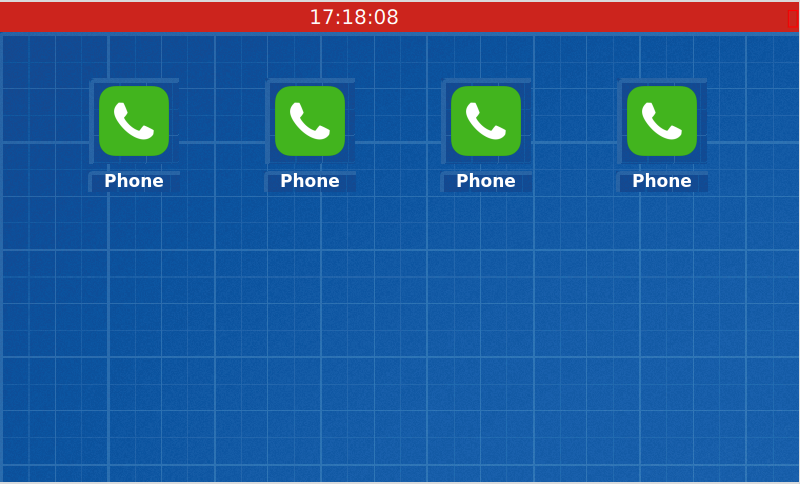
\includegraphics[width=\linewidth]{wm1}
\end{figure}

\end{frame}

%%%%%%%%%%%%%%%%%%%%%%%%%%%%%%%%%%%%%%%%%%%%%%%%%%%%%%%%%%%%%%%%%%%%%%%%%%%%%%%
%%%%%%%%%%%%%%%%%%%%%%%%%%%%%%%%%%%%%%%%%%%%%%%%%%%%%%%%%%%%%%%%%%%%%%%%%%%%%%%

\begin{frame}
\frametitle{Примеры работы}

\begin{figure}[h!]
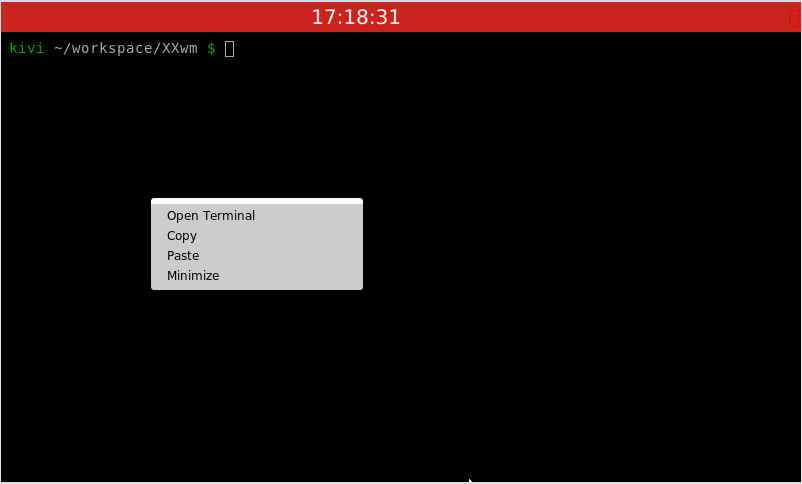
\includegraphics[width=\linewidth]{wm2}
\end{figure}

\end{frame}

%%%%%%%%%%%%%%%%%%%%%%%%%%%%%%%%%%%%%%%%%%%%%%%%%%%%%%%%%%%%%%%%%%%%%%%%%%%%%%%
%%%%%%%%%%%%%%%%%%%%%%%%%%%%%%%%%%%%%%%%%%%%%%%%%%%%%%%%%%%%%%%%%%%%%%%%%%%%%%%

\begin{frame}
\frametitle{Примеры работы}

\begin{figure}[h!]
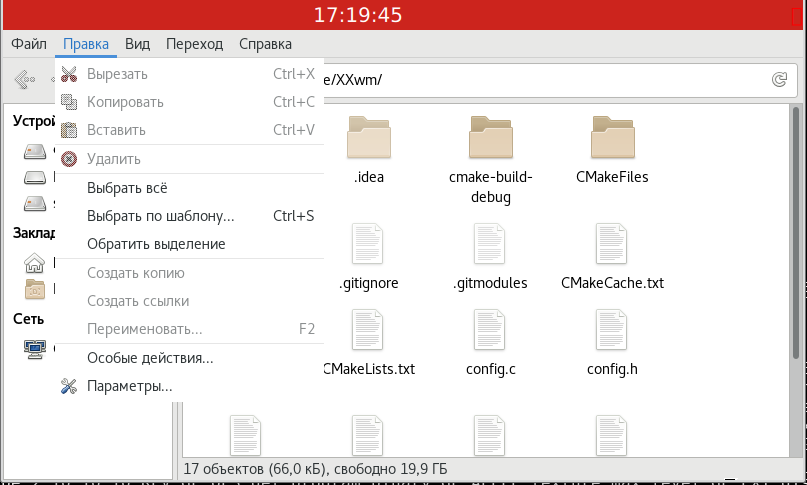
\includegraphics[width=\linewidth]{wm3}
\end{figure}

\end{frame}

%%%%%%%%%%%%%%%%%%%%%%%%%%%%%%%%%%%%%%%%%%%%%%%%%%%%%%%%%%%%%%%%%%%%%%%%%%%%%%%
%%%%%%%%%%%%%%%%%%%%%%%%%%%%%%%%%%%%%%%%%%%%%%%%%%%%%%%%%%%%%%%%%%%%%%%%%%%%%%%

\begin{frame}
\frametitle{Примеры работы}

\begin{figure}[h!]
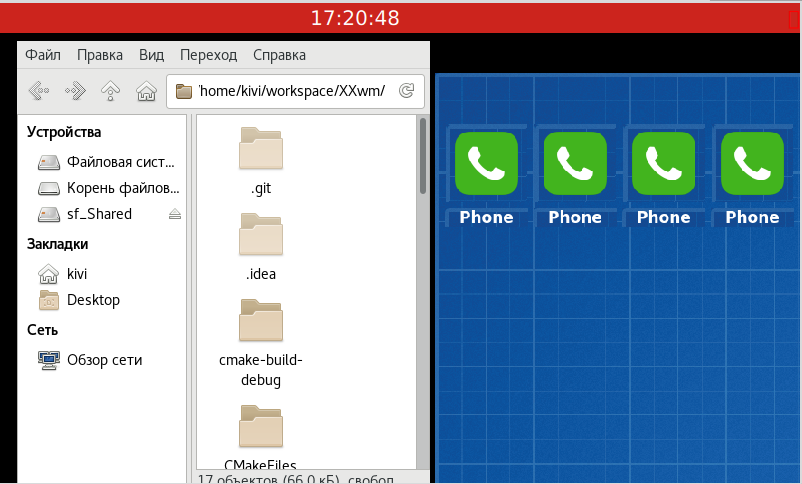
\includegraphics[width=\linewidth]{wm4}
\end{figure}

\end{frame}

%%%%%%%%%%%%%%%%%%%%%%%%%%%%%%%%%%%%%%%%%%%%%%%%%%%%%%%%%%%%%%%%%%%%%%%%%%%%%%%
%%%%%%%%%%%%%%%%%%%%%%%%%%%%%%%%%%%%%%%%%%%%%%%%%%%%%%%%%%%%%%%%%%%%%%%%%%%%%%%

\begin{frame}[fragile]
\frametitle{Добавление ОМ в экранный менеджер}

Необходимо поместить файл "ярлык" \texttt{xxwm.desktop} в \texttt{/usr/share/wayland-sessions/}
\begin{lstlisting}[style=crs_cpp]
[Desktop Entry]
Name=XXwm
Comment=Mobile Wayland window manager
Exec=~/workspace/XXwm/xxonwm
Type=Application
\end{lstlisting}

\end{frame}

%%%%%%%%%%%%%%%%%%%%%%%%%%%%%%%%%%%%%%%%%%%%%%%%%%%%%%%%%%%%%%%%%%%%%%%%%%%%%%%
%%%%%%%%%%%%%%%%%%%%%%%%%%%%%%%%%%%%%%%%%%%%%%%%%%%%%%%%%%%%%%%%%%%%%%%%%%%%%%%

\begin{frame}
\frametitle{Примеры работы}

\begin{figure}[h!]
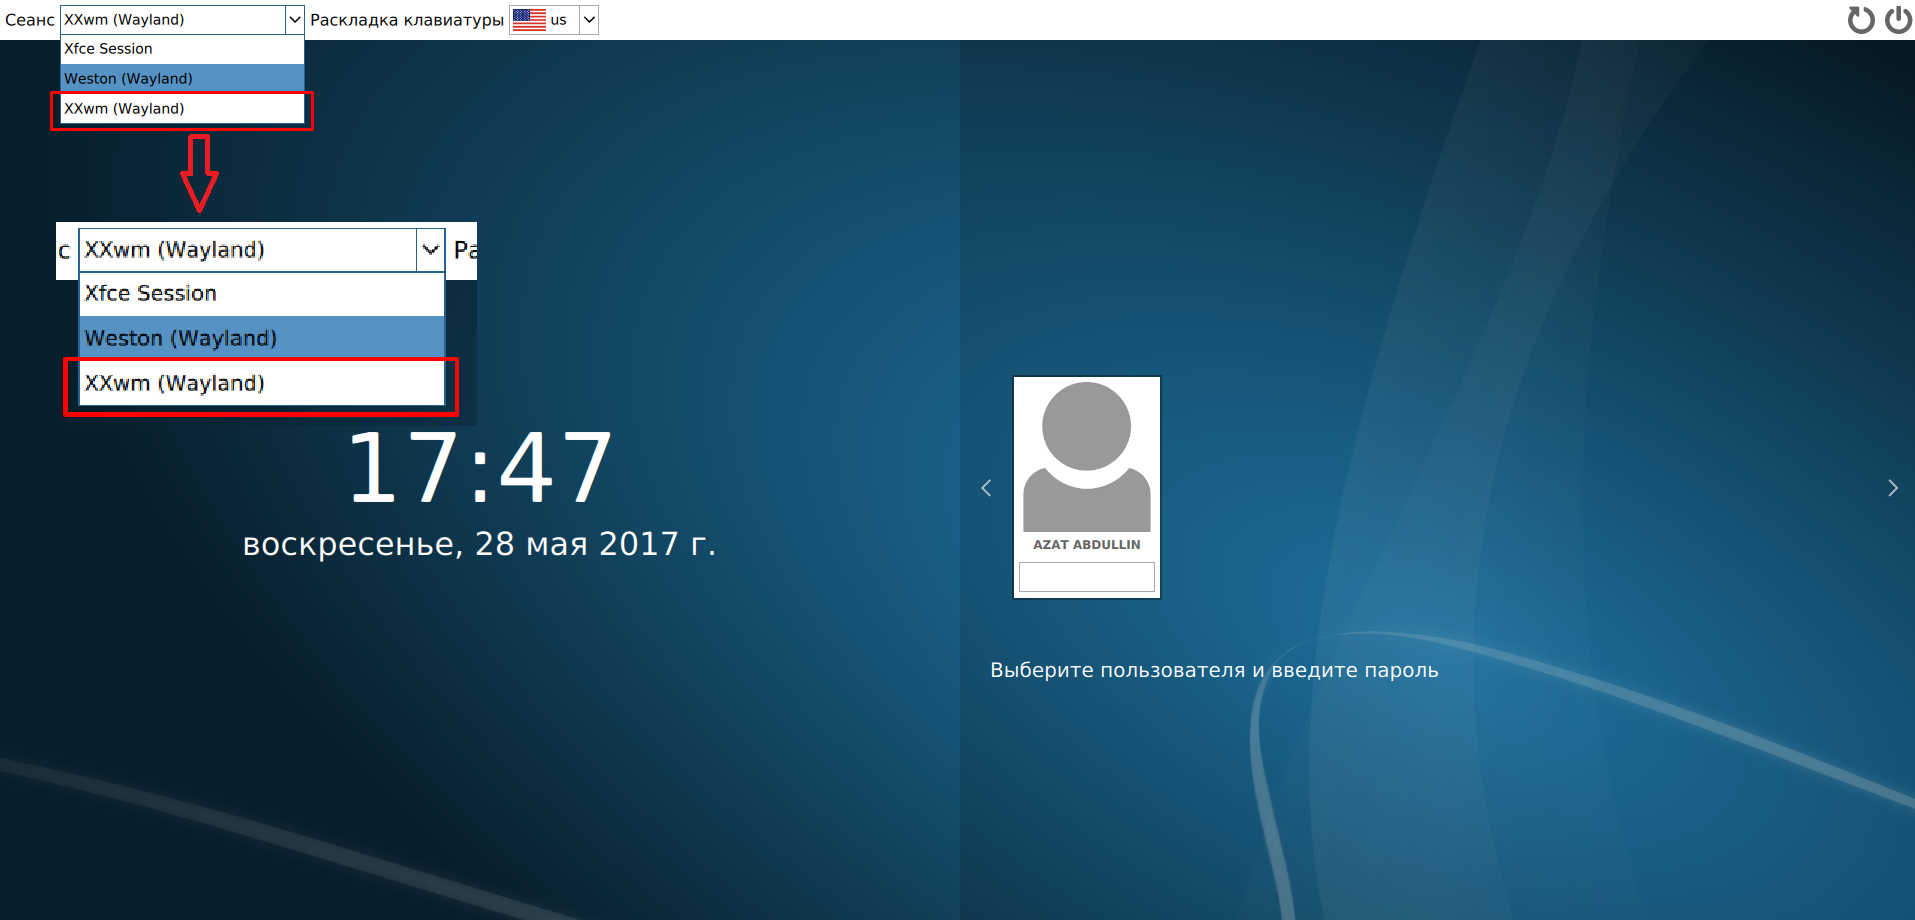
\includegraphics[width=\linewidth]{sddm}
\end{figure}

\end{frame}

%%%%%%%%%%%%%%%%%%%%%%%%%%%%%%%%%%%%%%%%%%%%%%%%%%%%%%%%%%%%%%%%%%%%%%%%%%%%%%%
%%%%%%%%%%%%%%%%%%%%%%%%%%%%%%%%%%%%%%%%%%%%%%%%%%%%%%%%%%%%%%%%%%%%%%%%%%%%%%%





